\chapter*{符號列表}
\label{chp:symbol}
% \addcontentsline{toc}{chapter}{符號列表}


%英文字母 -> 希臘字母%
%小寫 -> 大寫%
%向量 -> 純量% %粗->細%


% \section*{符號列表}
\subsection*{座標系}

\begin{longtable}[l]{cl}
    % $\text{Bell}(\cdot)$ & 鐘形函式\\
    $\boldsymbol{P}$ & 座標點\\
    $x,y,z$ & 座標點$\boldsymbol{P}$的$x,y,z$分量\\
    $\boldsymbol{V}$ & 單位向量\\
    $u,v,w$ & 單位向量$\boldsymbol{V}$的$x,y,z$分量\\
    $d,\alpha,\beta$ & 單位向量$\boldsymbol{V}$在球座標系中的天頂角(Zenith Angle)、方位角(Azimuth Angle)、距離分量\\
\end{longtable}

% \begin{figure}[ht]
% 	\centering
% 	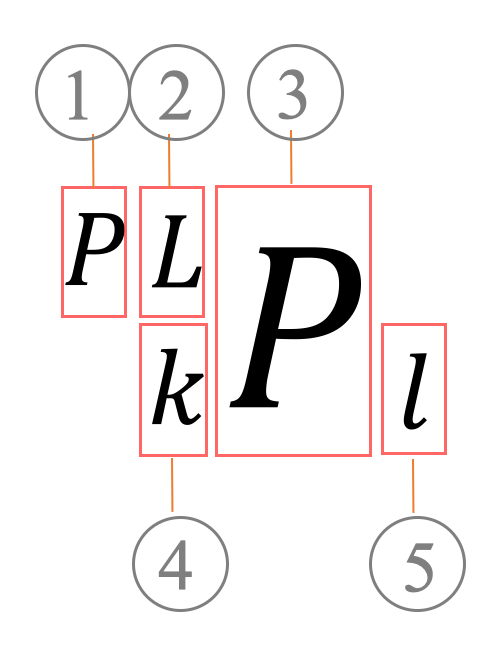
\includegraphics[width=3cm]{ch1pic/not_pos.png}
%     \caption{座標系小標解釋}
%     \label{pic:not_pos}
% \end{figure}

% \begin{description}
%     \item[(1)] 投影至的座標系($P$: PD座標系;$L$: LED座標系)
%     \item[(2)] 定義於哪個座標系($P$: PD座標系;$L$: LED座標系)
%     \item[(3)] 座標系符號(如上表)
%     \item[(4)] 第$k$個樣本點($k=1,2,...,K$)
%     \item[(5)] 第$l$個LED或第$p$個PD($l=1,2,...,L$;$p=1,2,...,P$)
% \end{description}



\onehalfspacing

\subsection*{座標系轉換}

\begin{longtable}[l]{cl}
    $\boldsymbol{H}=\left[\begin{array}{cc}
         \boldsymbol{Ro}  & \boldsymbol{T} \\
        0_{1\times3} & 1
        \end{array}\right]$ & 齊次轉換矩陣 Homogeneous Transformation Matrix\\
    $\boldsymbol{T}=\left[\begin{array}{ccc}t_x&t_y&t_z\end{array}\right]^T$ & 平移向量 Transfer Vector\\
    $\boldsymbol{T}^{sph}=\left[\begin{array}{ccc}t_d&t_{\alpha}&t_{\beta}\end{array}\right]^T$ & 平移向量以球座標系表示\\
    $\boldsymbol{Ro}=\left\{\gamma_{ij}\right\}$ & 旋轉矩陣 Rotation Matrix\\
\end{longtable}

% \begin{figure}[ht]
% 	\centering
% 	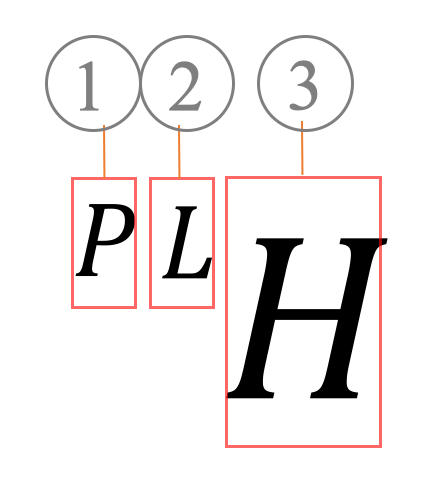
\includegraphics[width=3cm]{ch1pic/not_transform.png}
%     \caption{座標系轉換小標解釋}
%     \label{pic:not_transform}
% \end{figure}

% \begin{description}
%     \item[(1)] 投影至的座標系($P$: PD座標系;$L$: LED座標系)
%     \item[(2)] 定義於哪個座標系($P$: PD座標系;$L$: LED座標系)
%     \item[(3)] 座標系轉換符號(如上表)
%     \item[(4)] 第$k$個樣本點($k=1,2,...,K$)] 
% \end{description}




% \begin{figure}[ht]
% 	\centering
% 	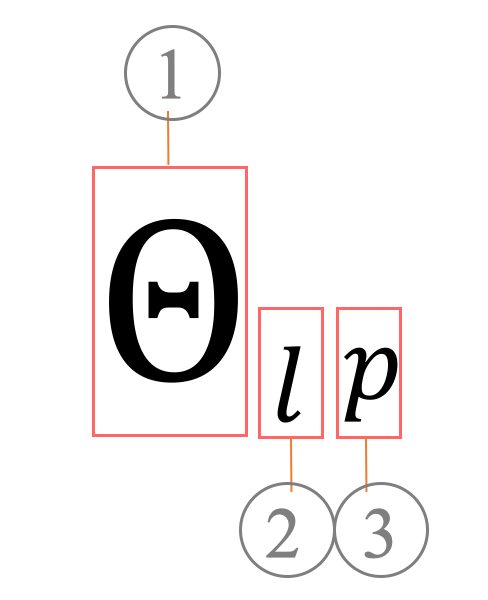
\includegraphics[width=3cm]{ch1pic/not_interactive.png}
%     \caption{LED與PD的交互關係小標解釋}
%     \label{pic:not_interactive}
% \end{figure}

% \begin{description}
%     \item[(1)] LED與PD的交互關係符號(如上表)
%     \item[(2)] 第$l$個LED($l=1,2,...,L$)
%     \item[(3)] 第$p$個PD($p=1,2,...,P$)
%     \item[(4)] 第$k$個樣本點($k=1,2,...,K$) 
% \end{description}

\onehalfspacing

\subsection*{硬體參數}

\begin{longtable}[l]{cl}
    % $\text{Bell}(\cdot)$ & 鐘形函式\\
    符號 & LED硬體參數\\ \hline
    $Ml$ & LED的朗伯次方(Lambertian Order)\\
    $Pt$ & 總輻射通量(Total Radiation Flux) 
\end{longtable}

\begin{longtable}[l]{cl}
    % $\text{Bell}(\cdot)$ & 鐘形函式\\
    符號 & PD硬體參數\\ \hline
    $Mp$ & PD的朗伯次方(Lambertian Order)\\
    $A$ & 有效面積\\
    $Re$ & 響應率(Responsivity)\\
    $s$ &飽和電流
\end{longtable}


\onehalfspacing

\subsection*{LED與PD的交互關係}

\begin{longtable}[l]{cl}
    % $\text{Bell}(\cdot)$ & 鐘形函式\\
    $\phi$ & PD入射角\\
    $\theta$ & LED出射角\\
    $D$&距離\\
\end{longtable}

\onehalfspacing

\subsection*{光學領域單位}

\begin{longtable}[l]{cllll}
    % $\text{Bell}(\cdot)$ & 鐘形函式\\
    符號& 中文& 英文 & 單位符號&國際單位制\\\hline
    $\Omega$ & 立體角&Solid Angle& $sr$&球面度(Steradian) \\
    $\omega$ & 角度&Angle& $rad$&弧度(radian)\\
    $r$ & 半徑&Radius&  $m$ &公尺\\
    $\Phi$ & 輻射通量&Radiation Flux& $W$&瓦特(Watt)\\
    $I$ & 輻射強度&Radiation Intensity & $W\cdot sr^{-1}$&瓦特每球面度 \\
    $E$ & 輻照度&Irradiance&$W\cdot m^{-2}$ &瓦特每平方公尺\\
\end{longtable}


\onehalfspacing

\subsection*{系統與演算法}

\begin{longtable}[l]{cl}
    % $\text{Bell}(\cdot)$ & 鐘形函式\\
    $t_d$ & 兩座標系之間距離\\
    $\boldsymbol{Tv}$ & 兩座標系中對方所在方位\\
    $L,P$ & LED與PD總數\\
    $l,p$ & LED與PD編號\\
    $Fl,Fp$ & 過濾後的LED與PD數量\\
    $Ra$& 餘弦比值\\
    $r_c$& 取作餘弦比值參考值的硬體編號\\
    $r_s$& 參考平面由$r_c$與$r_s$編號的硬體資訊獲得\\
    $N$& 平面法向量\\

\end{longtable}




\onehalfspacing

\section*{小標解釋}

論文中由於座標系、硬體數量、樣本數量眾多,為了區分不同上下小標的意義,以圖\ref{pic:symbol}呈現各小標意思,左上標表示座標系,左下標顯示是哪個樣本,而右下標則依照物理量代表著LED或PD的編號,在LED與PD交互關係的物理量中右下標同時包含兩者的編號。

\begin{figure}[ht]
	\centering
	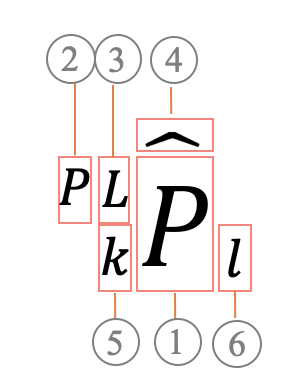
\includegraphics[width=2cm]{ch1pic/not_whole.png}
    \caption{符號小標解釋}
    \label{pic:symbol}
\end{figure}



\begin{description}
    \item[(1) 符號] 
    \item[(2) 投影至的座標系:] ($P$: PD座標系;$L$: LED座標系)
    \item[(3) 定義於哪個座標系:] ($P$: PD座標系;$L$: LED座標系)
    \item[(4) 量測訊號:] $\hat{(\cdot)}$代表該物理量為量測所得或處理量測所得訊號而得
    \item[(5) 樣本點:] 第$k$個樣本點($k=1,2,...,K$)
    \item[(6) 硬體編號:] 第$p$個PD($p=1,2,...,P$)或第$l$個LED($l=1,2,...,L$);LED與PD交互關係物理量的(6)小標為$lp$兩者的交互關係
    \item[(7) 使用的座標系統:]  以何種座標系呈現(無:卡氏座標系;$sph$:球座標系)
\end{description}


以下舉例解釋:
\begin{description}
\item[- $^{PL}_{k}\hat{\boldsymbol{T}}$:]第k個樣本點中,模擬量測方式所得到的PD座標系指向LED座標系的平移向量。

\item[- $^{L}P_l,^{PL}P_l$:]$^{L}P_l,$為第l個LED於LED座標系上的位置座標,$^{PL}P_l$則是將其投影到PD座標系上

\item[- $_{k}D_lp$:]第k個樣本點鐘,第l個LED與第p個PD的距離
$Ml_l$:第l個LED的朗博次方
\end{description}